\documentclass[10pt,conference]{IEEEtran}

\usepackage{cite}
\usepackage{amsmath,amssymb,amsfonts}
\usepackage{algorithmic}
\usepackage{graphicx}
\graphicspath{{figures/}}
\setkeys{Gin}{draft=false}
\usepackage{textcomp}
\usepackage{xcolor}
\usepackage{listings}
\usepackage{booktabs}
\usepackage{placeins}
\usepackage{makecell}
\usepackage{tabularx}
\usepackage{array}
\usepackage{flafter}
\usepackage{float}
\usepackage{url}
\usepackage[final]{microtype}
\emergencystretch=1em
\newcommand{\method}{ReFCode}
\newcommand{\best}[1]{\textbf{#1}}
\newcommand{\second}[1]{\underline{#1}}
\usepackage[caption=false,font=footnotesize]{subfig}
\usepackage{needspace}

\newcolumntype{L}{>{\raggedright\arraybackslash}X}
\newcolumntype{C}{>{\centering\arraybackslash}p{0.073\columnwidth}}

\lstdefinestyle{failurecaseclean}{
    language=Python,
    basicstyle=\ttfamily\footnotesize,
    keywordstyle=\bfseries,
    commentstyle=\itshape\color{gray!70!black},
    stringstyle=\color{black},
    showstringspaces=false,
    columns=fullflexible,
    keepspaces=true,
    breaklines=true,
    frame=none,
    aboveskip=0pt,
    belowskip=0pt,
    xleftmargin=0pt,
    xrightmargin=0pt,
    escapeinside={(*@}{@*)}
}
% Float spacing and placement controls.
% Keep IEEE-style top/bottom floats, but avoid packing too many tables/figures on one page.
\setlength{\textfloatsep}{9pt plus 2pt minus 2pt}
\setlength{\dbltextfloatsep}{9pt plus 2pt minus 2pt}
\setlength{\intextsep}{8pt plus 2pt minus 2pt}
\setlength{\floatsep}{8pt plus 2pt minus 2pt}
\setcounter{topnumber}{2}
\setcounter{bottomnumber}{1}
\setcounter{totalnumber}{3}
\renewcommand{\topfraction}{0.82}
\renewcommand{\bottomfraction}{0.45}
\renewcommand{\dbltopfraction}{0.88}
\renewcommand{\textfraction}{0.12}
\renewcommand{\floatpagefraction}{0.75}
\renewcommand{\dblfloatpagefraction}{0.75}

% Finding and answer boxes.
% Finding: light orange; Answer: light green.
\definecolor{findingbg}{RGB}{255,247,235}
\definecolor{findingborder}{RGB}{224,154,87}
\definecolor{answerbg}{RGB}{240,250,242}
\definecolor{answerborder}{RGB}{102,168,117}

\newcommand{\resultbox}[4]{%
\vspace{3pt}
\noindent
\begingroup
\setlength{\fboxrule}{0.45pt}%
\setlength{\fboxsep}{4pt}%
\fcolorbox{#2}{#1}{%
\begin{minipage}{0.965\columnwidth}

\textbf{#3.} #4
\end{minipage}%
}%
\endgroup
\vspace{4pt}
}

\newcommand{\findingbox}[2]{%
\resultbox{findingbg}{findingborder}{#1}{#2}%
}

\newcommand{\answerbox}[2]{%
\resultbox{answerbg}{answerborder}{Answer to #1}{#2}%
}

\definecolor{codegray}{RGB}{248,248,248}

\lstdefinestyle{failurecase}{
    basicstyle=\ttfamily\scriptsize,
    showstringspaces=false,
    columns=fullflexible,
    keepspaces=true,
    breaklines=true,
    frame=none,
    aboveskip=0pt,
    belowskip=0pt,
    xleftmargin=0pt,
    xrightmargin=0pt,
    escapeinside={(*@}{@*)}
}

\lstdefinestyle{failurecase}{
    basicstyle=\ttfamily\scriptsize,
    columns=fullflexible,
    keepspaces=true,
    breaklines=true,
    showstringspaces=false,
    frame=none,
    backgroundcolor=\color{codegray},
    aboveskip=0pt,
    belowskip=0pt,
    xleftmargin=2pt,
    xrightmargin=2pt,
    escapeinside={(*@}{@*)}
}

\newcommand{\failurelisting}[3]{%
\vspace{5pt}
\refstepcounter{lstlisting}\label{#1}%
\noindent{\footnotesize Listing~\thelstlisting. #2}
\vspace{4pt}

\noindent\hrule
\vspace{4pt}
#3
\vspace{2pt}
\noindent\hrule
\vspace{5pt}
}

\def\BibTeX{{\rm B\kern-.05em{\sc i\kern-.025em b}\kern-.08em
    T\kern-.1667em\lower.7ex\hbox{E}\kern-.125emX}}

\begin{document}

\title{\method{}: Failure-Calibrated Dual-Granularity Refinement for Code Search}

\author{\IEEEauthorblockN{Anonymous Author(s)}}

\maketitle

\begin{abstract}
Code search is a fundamental task in software development, aiming to retrieve code snippets that match developers' natural language queries. Recent contrastive-learning-based methods have improved code search by learning aligned query-code representations and incorporating hard negative samples. However, such hard negatives are usually constructed as training-time proxies for difficulty, and may not reflect the high-ranked misleading candidates produced by a trained retriever during inference. Our empirical study shows that strong retrievers still produce retrieved-but-mis-ranked cases, where the ground-truth code is recalled within the top-\(K\) candidates but suppressed by incorrect high-ranked results. We further observe that model-induced high-ranked candidates are not well aligned with conventional static hard negatives. Motivated by these findings, we propose ReFCode, a failure-calibrated dual-granularity refinement framework for code search. ReFCode harvests top-ranked non-ground-truth candidates from an initial retriever and uses them as targeted supervision for global contrastive refinement. It further incorporates lightweight local interaction to capture fine-grained query-code differences and fuses global and local scores for final ranking. Experiments on the six-language CodeSearchNet benchmark show that ReFCode achieves an average MRR of 81.2\%, outperforming the strongest baseline by 0.9 MRR points. Ablation studies and ranking behavior analysis further validate the effectiveness of failure-calibrated supervision, local interaction, and global-local fusion.
\end{abstract}

\begin{IEEEkeywords}
Code search, contrastive learning, failure-calibrated refinement, dual-granularity ranking
\end{IEEEkeywords}

\section{Introduction}

Code search plays a critical role in modern software development by helping developers locate reusable code snippets from large-scale repositories. Given a natural language query, the goal of code search is to retrieve code snippets that best match the developer's intent. With the rapid growth of open-source software and the increasing complexity of software systems, effective code search has become a fundamental technique for program comprehension, software reuse, and development assistance~\cite{CodeSearchSurvey,CodeSearchNet}. Recent advances in pre-trained code models have substantially improved code search by learning semantic representations of natural language descriptions and source code in a shared embedding space~\cite{CodeBERT,GraphCodeBERT,UniXcoder}.

Most neural code search methods follow a dual-encoder retrieval paradigm. A query encoder and a code encoder separately map natural language queries and code snippets into a shared representation space, and retrieval is performed by ranking candidate code snippets according to their representation similarity~\cite{CodeBERT,GraphCodeBERT,UniXcoder,CoCoSoDa}. To improve the discriminative ability of such representations, recent studies have introduced contrastive learning and hard negative sampling, where semantically close but mismatched query-code pairs are used to sharpen the decision boundary between relevant and irrelevant candidates~\cite{CodeRetriever,CoCoSoDa,AAAIUA,CoCoHaNeRe,HedgeCode}. These methods have shown strong retrieval performance and have become a common training strategy for modern neural code search models.

Despite this progress, existing contrastive code search methods usually construct supervision from training-time negative candidates rather than from the ranked results produced by the trained retriever. These candidates are typically constructed according to lexical overlap, representation similarity, or batch-level sampling. Although they expose the model to more informative negative pairs and improve representation learning, the constructed candidates may not reflect the high-ranked misleading candidates observed during inference. In other words, a model can be trained to distinguish training-time hard negatives while still assigning high ranks to incorrect candidates in its final retrieval results. This supervision mismatch leaves an important gap between training-time optimization and the ranking behavior observed during inference.

This gap is particularly important for code search because retrieval quality is determined by the relative order of candidates in the final ranked list. A high-ranked incorrect candidate can directly suppress the ground-truth code, even when the model has learned generally effective global representations. Therefore, the key limitation is not only whether a negative sample is hard during training, but whether the model is exposed to the high-ranked incorrect candidates that it actually retrieves. From this perspective, model-induced high-ranked candidates and ranking errors provide more direct signals for understanding and improving the ranking behavior of a code search model. Fig.~\ref{fig:topk_failure} illustrates the difference between retrieval coverage and top-ranked ordering correctness. Although the ground-truth code $c^{+}$ appears within the top-$K$ candidate set, a high-ranked incorrect candidate $c^{-}$ may still precede it, resulting in a retrieved-but-mis-ranked failure.

To examine this issue, we conduct an empirical study on the retrieval behavior of strong code search models. The study shows that a non-negligible portion of queries remains affected by high-ranked retrieval failures, even when the initial retriever already achieves strong overall performance. In many cases, incorrect candidates are ranked above the ground-truth code, or the ground-truth code is retrieved but not ranked at the top. More importantly, model-induced high-ranked candidates are not well aligned with conventional static hard negatives, suggesting that training-time hard candidates do not sufficiently characterize the errors that affect final ranking. These findings lead to the research question studied in this paper: how can a code search model learn from its own retrieval failures?

To address this question, we propose \method{}, a failure-calibrated dual-granularity refinement framework for code search. Instead of relying only on pre-defined hard candidates, \method{} first uses a strong initial retriever to harvest top-ranked non-ground-truth candidates from its own ranked results. These model-induced high-ranked candidates are then used to construct failure-calibrated supervision, enabling the model to calibrate its decision boundary around candidates that are closer to inference-time ranking errors. Beyond global semantic matching, \method{} further introduces dual-granularity refinement by incorporating local interaction between queries and code snippets. Finally, global-local fusion combines the efficiency of global retrieval with the fine-grained matching ability of local interaction to improve the final ranking.

We evaluate \method{} on the six-language CodeSearchNet benchmark. Experimental results show that \method{} achieves the highest average MRR among all compared methods and further improves a strong initial retriever. Ablation studies and ranking behavior analysis further validate the contributions of failure-calibrated supervision, local interaction, and global-local fusion in improving the final ranking.

The main contributions of this paper are summarized as follows:

\begin{itemize}
    \item We reveal a supervision mismatch in hard-negative-based code search: statically constructed hard negatives are not well aligned with the model-induced high-ranked candidates produced by trained retrievers. Based on this finding, we identify model-induced high-ranked candidates as targeted supervision signals for code search refinement.
    
    \item We propose \method{}, a failure-calibrated dual-granularity refinement framework for code search. \method{} learns from high-ranked non-ground-truth candidates exposed by the initial retriever and calibrates ranking decisions through dual-granularity refinement, enabling the model to combine global semantic matching with local interaction.
    
    \item We validate \method{} on the six-language CodeSearchNet benchmark. The results show that \method{} achieves the best average MRR among representative code search methods, while ablation studies and ranking behavior analysis further validate the contributions of failure-calibrated supervision, local interaction, and global-local fusion to ranking refinement.
\end{itemize}

% \begin{figure}[t]
%     \centering
%     \includegraphics[draft=false,width=\columnwidth]{figures/editable_topk_diagram.pdf}
%     \caption{Motivating illustration of high-ranked retrieval behavior. The ground-truth code $c^{+}$ can be retrieved within the top-$K$ candidate set, but a high-ranked incorrect candidate $c^{-}$ may still be ranked above it, leading to a retrieved-but-mis-ranked failure.}
%     \label{fig:topk_failure}
% \end{figure}

\begin{figure}[t]
\centering

\subfloat[Retrieved in top-\(K\)]{
    \includegraphics[
        width=0.46\columnwidth,
        trim=5 10 510 32,
        clip
    ]{editable_topk_diagram.pdf}
}
\hfill
\subfloat[Retrieved but mis-ranked]{
    \includegraphics[
        width=0.46\columnwidth,
        trim=510 10 5 32,
        clip
    ]{editable_topk_diagram.pdf}
}

\caption{Motivating illustration of high-ranked retrieval behavior. 
The ground-truth code \(c^{+}\) can be retrieved within the top-\(K\) candidate set, but a high-ranked incorrect candidate \(c^{-}\) may still be ranked above it, leading to a retrieved-but-mis-ranked failure.}
\label{fig:topk_failure}
\end{figure}

\section{Empirical Study}

Before presenting our approach, we first examine why a strong code search retriever still needs refinement. Existing hard-negative-based methods usually construct difficult candidates before or during training, but the candidates that affect the final ranked list are produced by the trained retriever itself. This section studies model-induced high-ranked errors and candidates, and examines how they differ from training-time hard negatives constructed by prior methods.

\subsection{Study Design}

We conduct the study on CodeSearchNet~\cite{CodeSearchNet} under the standard natural language code search setting. For each query, a trained dual-encoder retriever produces a ranked list of candidate code snippets according to representation similarity. We analyze this ranked list from three perspectives: whether the ground-truth code is recalled but mis-ranked, how statically mined hard negatives align with top-ranked non-ground-truth candidates produced by the retriever, and whether high-ranked misleading candidates involve fine-grained semantic differences that affect ranking correctness.

Fig.~\ref{fig:topk_failure} illustrates the core failure mode studied in this section. The left panel shows that coarse retrieval can already succeed, where the ground-truth code $c^{+}$ is retrieved into the top-$K$ neighborhood of the query $q$. However, the right panel shows that successful recall does not necessarily imply correct top-ranked ordering. A high-ranked incorrect candidate $c^{-}$ may still be placed closer to the query and ranked above $c^{+}$, resulting in a retrieved-but-mis-ranked failure. This distinction is important because such failures are not complete retrieval misses, but ranking errors inside the high-ranked candidate space.

Given a query $q_i$, its ground-truth code snippet $c_i^{+}$, and the ranked candidate list returned by the retriever, we use retrieval failure to describe model-induced ranking errors exposed in the retrieved list. At the candidate level, a retrieval failure refers to a non-ground-truth candidate $c^{-}$ that is ranked above $c_i^{+}$. At the query level, we focus on retrieved-but-mis-ranked cases, where $c_i^{+}$ appears within the top-$K$ candidate set but is not ranked first. These definitions allow us to quantify ranking errors that directly affect the final order and to analyze their relation to training-time hard candidates.

Rather than evaluating end-to-end performance, this analysis characterizes retrieval behavior. We analyze retrieval outcomes on the test split and negative-sample alignment on the training split, comparing training-time hard candidates with high-ranked candidates induced by the trained retriever.

\subsection{High-Ranked Retrieval Failures}

Fig.~\ref{fig:topk_failure} shows that a strong retriever may already place the relevant code in the high-ranked candidate space, yet still rank a misleading candidate above it. Therefore, the key question is whether the retriever can correctly order semantically close candidates near the top of the ranked list.

Table~\ref{tab:retrieval_outcomes} reports the distribution of retrieval outcomes across the six CodeSearchNet languages. Top-1 denotes cases where the ground-truth code is ranked first, Gold@2--50 denotes retrieved-but-mis-ranked cases within the top-50 candidates, and Not in Top-50 denotes cases where the ground-truth code is outside the top-50 list. The Gold@2--50 proportion remains substantial, reaching 36.5\% on PHP, 31.9\% on Python, 30.5\% on JavaScript, and 30.3\% on Java; even Go still has 11.0\%.

\begin{table}[t]
\centering
\caption{Distribution of retrieval outcomes across CodeSearchNet languages.}
\label{tab:retrieval_outcomes}
\footnotesize
\setlength{\tabcolsep}{4.2pt}
\renewcommand{\arraystretch}{1.10}
\begin{tabular*}{0.95\columnwidth}{@{\extracolsep{\fill}}lccc@{}}
\toprule
Language & Top-1 & Gold@2--50 & Not in Top-50 \\
\midrule
Java       & 67.2 & 30.3 & 2.5 \\
JavaScript & 67.4 & 30.5 & 2.1 \\
Ruby       & 73.0 & 26.1 & 0.9 \\
Python     & 67.0 & 31.9 & 1.1 \\
PHP        & 61.3 & 36.5 & 2.2 \\
Go         & 88.5 & 11.0 & 0.5 \\
\midrule
Avg.       & 70.7 & 27.7 & 1.6 \\
\bottomrule
\end{tabular*}
\end{table}

This observation indicates that many code search errors are not caused by the retriever completely missing the relevant code. Instead, the retriever has often captured coarse-grained relevance by placing the ground-truth code near the top of the ranked list, but still assigns higher ranks to misleading alternatives. Such cases expose ranking errors within a semantically related candidate set.

\findingbox{Finding 1: High-Ranked Retrieval Failures}{Strong retrievers still produce a substantial number of retrieved-but-mis-ranked cases. The ground-truth code is often recalled within the top-50 candidates but is suppressed by high-ranked incorrect results, suggesting that code search errors are frequently ranking failures rather than complete retrieval misses.}

\subsection{Mismatch with Static Hard Negatives}

Table~\ref{tab:negative_alignment} compares random negatives, statically mined hard negatives, and model-induced candidates. 
Random negatives represent conventional easy negatives, while Static HN denotes statically mined hard negatives constructed by predefined mining strategies. 
Model-Induced Cand. denotes top-ranked non-ground-truth candidates produced by the trained initial retriever. 
Score Gap measures how close a negative candidate is to the ground-truth code; a smaller gap indicates a harder candidate. 
Top-50 Cov. measures the proportion of candidates appearing in the retriever's top-50 ranked list, while Cand. Overlap measures the overlap with model-induced candidates.

\begin{table}[t]
\centering
\caption{Alignment between static negatives and model-induced candidates.}
\label{tab:negative_alignment}
\footnotesize
\setlength{\tabcolsep}{4.2pt}
\renewcommand{\arraystretch}{1.10}
\begin{tabular*}{0.95\columnwidth}{@{\extracolsep{\fill}}lccc@{}}
\toprule
Candidate Type & Score Gap & Top-50 Cov. & Cand. Overlap \\
\midrule
Random Neg.           & 0.608 & 0.001 & 0.001 \\
Static HN             & 0.350 & 0.085 & 0.085 \\
Model-Induced Cand.   & 0.120 & 1.000 & --    \\
\bottomrule
\end{tabular*}
\end{table}


As shown in Table~\ref{tab:negative_alignment}, static hard negatives are substantially more difficult than random negatives, reducing the score gap from 0.608 to 0.350. 
However, their top-50 coverage and overlap with model-induced candidates are only 0.085, indicating that most statically mined hard negatives do not appear among the high-ranked non-ground-truth candidates produced by the trained retriever. 
In contrast, model-induced candidates have the smallest score gap of 0.120. 
Their top-50 coverage is 1.000 by construction, since they are collected from the retriever's top-ranked results.

This mismatch indicates that static hard negatives can improve sample difficulty, but they do not sufficiently characterize the high-ranked non-ground-truth candidates induced by the trained retriever in its own ranked results.

\findingbox{Finding 2: Supervision Mismatch with Static Hard Negatives}{Statically mined hard negatives are not well aligned with the model-induced high-ranked candidates produced by the trained retriever. This mismatch indicates that training-time sample difficulty and the model's own ranking difficulty are not equivalent.}

% \begin{figure}[!t]
% \centering
% \begin{minipage}{\linewidth}

% \refstepcounter{lstlisting}\label{lst:flip_case}
% \noindent{\footnotesize Listing~\thelstlisting. API-level mismatch in a high-ranked misleading candidate.}
% \vspace{3pt}

% \noindent\hrule
% \vspace{3pt}
% \begin{lstlisting}[style=failurecase]
% (*@\textit{Query: Vertically flip the given PIL image.}@*)

% (*@\textbf{Ground-truth code}@*)
% def vflip(img):
%     return img.transpose(Image.FLIP_TOP_BOTTOM)

% (*@\textbf{Top-ranked misleading candidate}@*)
% def hflip(img):
%     return img.transpose(Image.FLIP_LEFT_RIGHT)
% \end{lstlisting}
% \vspace{2pt}
% \noindent\hrule

% \end{minipage}
% \end{figure}

\subsection{Fine-Grained Misleading Candidates}

Listing~\ref{lst:flip_case} presents a representative high-ranked misleading candidate. 
In this case, the query asks for vertically flipping a given PIL image. 
The ground-truth code and the top-ranked candidate share almost the same function structure and use the same image transformation API, but their intended operations differ in a key API-level argument: the ground-truth code uses \texttt{Image.FLIP\_TOP\_BOTTOM}, whereas the misleading candidate uses \texttt{Image.FLIP\_LEFT\_RIGHT}. 
This local difference changes the functional semantics from vertical flipping to horizontal flipping. 
Although both snippets are globally similar and rely on the same API call pattern, the correctness of the result is determined by a single local argument.

% \begin{figure}[!t]
% \centering
% \begin{minipage}{\linewidth}
% \refstepcounter{lstlisting}\label{lst:clone_case}
% \noindent{\footnotesize Listing~\thelstlisting. Semantic mismatch between globally similar clone functions.}
% \vspace{3pt}

% \noindent\hrule
% \vspace{3pt}
% \begin{lstlisting}[style=failurecase]
% (*@\textit{Query: Clones object properties onto a new object.}@*)

% (*@\textbf{Ground-truth code}@*)
% function clone(obj) {
%     var newObj = {};
%     for (var prop in obj) newObj[prop] = obj[prop];
%     return newObj;
% }

% (*@\textbf{Top-ranked misleading candidate}@*)
% function cloneObject(obj) {
%     var temp = obj.constructor();
%     for (var key in obj) temp[key] = cloneObject(obj[key]);
%     return temp;
% }
% \end{lstlisting}
% \vspace{2pt}
% \noindent\hrule
% \end{minipage}
% \end{figure}

Listing~\ref{lst:clone_case} shows another case where the query asks for cloning object properties onto a new object. 
The top-ranked candidate is also a clone-related function, but it recursively clones nested objects, while the ground-truth implementation copies top-level properties into a new object. 
Although the two snippets are globally similar, the local implementation behavior differs from the query intent. 


These cases indicate that high-ranked misleading candidates are difficult to distinguish using only a single global representation. 
They are often close to the ground-truth code in lexical form or overall structure, but their functional behavior is determined by local implementation details. 
Fine-grained semantic differences may appear in API arguments, recursive behavior, object fields, control flow, or other local program elements that determine functional behavior.

\findingbox{Finding 3: Fine-Grained Misleading Candidates}{High-ranked misleading candidates are often not arbitrary mismatches. They can share similar APIs, lexical patterns, or program structures with the ground-truth code, while differing in local semantic details that determine functional correctness.}

\noindent\begin{minipage}{\linewidth}
\refstepcounter{lstlisting}\label{lst:flip_case}
\noindent{\footnotesize Listing~\thelstlisting. API-level mismatch in a high-ranked misleading candidate.}
\vspace{2pt}

\noindent\hrule
\vspace{2pt}
\begin{lstlisting}[style=failurecase]
(*@\textit{Query: Vertically flip the given PIL image.}@*)

(*@\textbf{Ground-truth code}@*)
def vflip(img):
    return img.transpose(Image.FLIP_TOP_BOTTOM)

(*@\textbf{Top-ranked misleading candidate}@*)
def hflip(img):
    return img.transpose(Image.FLIP_LEFT_RIGHT)
\end{lstlisting}
\vspace{1pt}
\noindent\hrule

\vspace{5pt}

\refstepcounter{lstlisting}\label{lst:clone_case}
\noindent{\footnotesize Listing~\thelstlisting. Semantic mismatch between globally similar clone functions.}
\vspace{2pt}

\noindent\hrule
\vspace{2pt}
\begin{lstlisting}[style=failurecase]
(*@\textit{Query: Clones object properties onto a new object.}@*)

(*@\textbf{Ground-truth code}@*)
function clone(obj) {
    var newObj = {};
    for (var prop in obj) newObj[prop] = obj[prop];
    return newObj;
}

(*@\textbf{Top-ranked misleading candidate}@*)
function cloneObject(obj) {
    var temp = obj.constructor();
    for (var key in obj) temp[key] = cloneObject(obj[key]);
    return temp;
}
\end{lstlisting}
\vspace{1pt}
\noindent\hrule
\end{minipage}
\vspace{4pt}

\subsection{Design Implications}

The three findings above lead to the design of \method{}. First, since many errors occur within the high-ranked candidate space, refinement should focus on candidates produced by the retriever rather than only improving coarse retrieval from the entire codebase. Second, since static hard negatives are weakly aligned with model-induced high-ranked candidates, refinement supervision should be constructed from the retriever's own ranked results. Third, since high-ranked misleading candidates often differ from the ground-truth code in local semantics, global representation refinement should be complemented with fine-grained query-code interaction. These implications motivate the failure candidate harvesting, failure-calibrated global refinement, and dual-granularity ranking components that form the core design of \method{}.



\section{Approach}
\label{sec:approach}

\subsection{Overview}
\label{sec:approach_overview}

The empirical study motivates a failure-calibrated view of code search. A strong dual-encoder retriever can place semantically related code snippets near the top of the ranked list, but high-ranked non-ground-truth candidates may still interfere with the final ordering. This suggests that refinement should not only improve coarse retrieval from the entire codebase, but also focus on candidates that the retriever itself already considers highly relevant.

\method{} follows a two-stage refinement process. It first mines top-ranked non-ground-truth candidates from the ranked results of an initial retriever. These candidates are then used as failure candidates for training a refined dual-granularity ranking model. The global branch provides the main contrastive refinement signal over pooled query--code representations, while the local branch provides an auxiliary late-interaction objective over the same sampled candidates. During inference, the refined global retriever retrieves a compact candidate set, and global-local fusion reranks the candidates to produce the final ranking for each query.

As shown in Fig.~\ref{fig:refcode_framework}, \method{} consists of three main components: failure candidate harvesting, failure-calibrated training, and dual-granularity reranking. The first component constructs model-induced failure candidates from the initial ranked lists. The second component optimizes a global contrastive objective together with an auxiliary local-interaction objective. The third component applies local matching only to the high-ranked candidates returned by the refined retriever and fuses the two scores for reranking. Compared with static hard negatives, the mined candidates are derived from the retriever's own ranking behavior rather than from external mining heuristics.

\begin{figure*}[t]
\centering
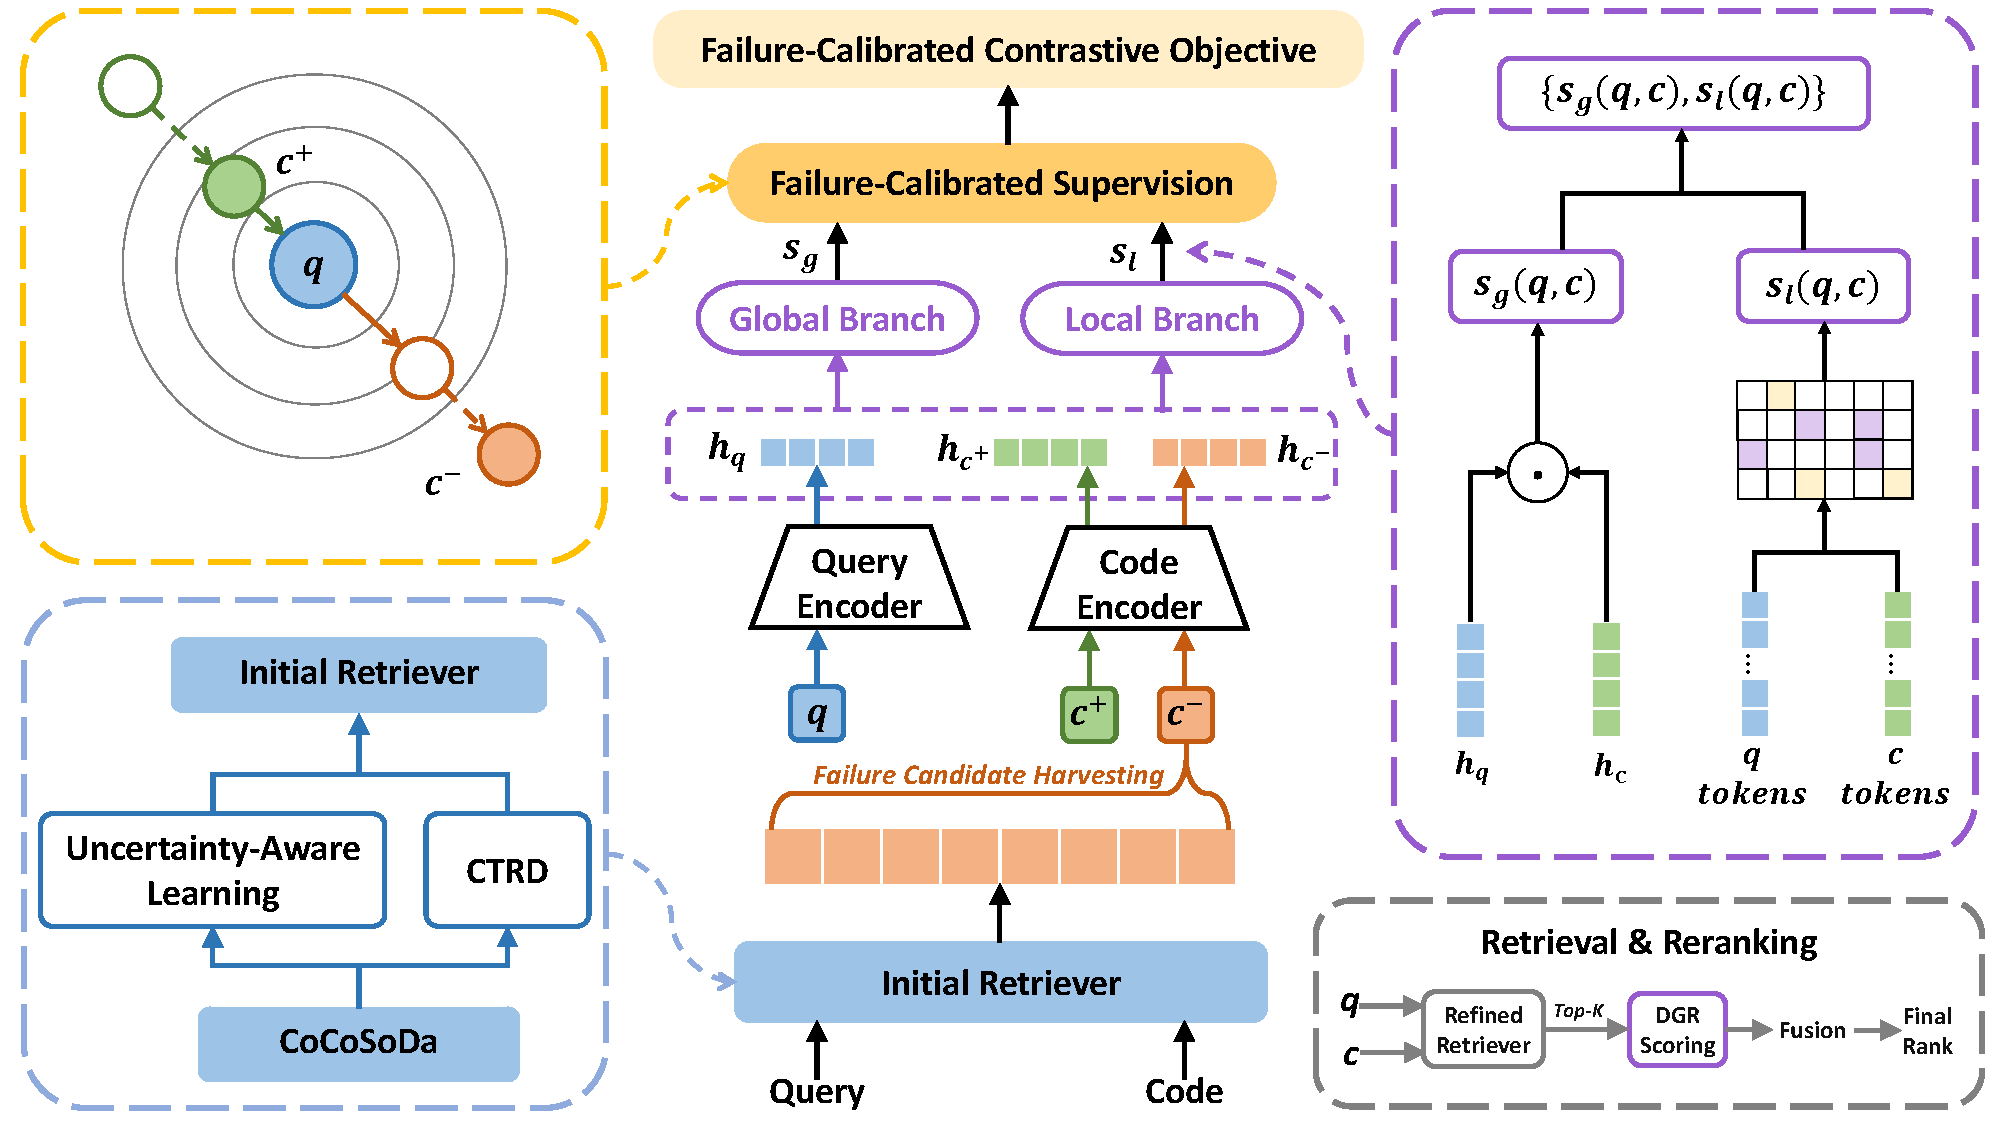
\includegraphics[width=\textwidth]{ReFCode_Framework.pdf}
\caption{Overview of ReFCode. ReFCode first mines top-ranked non-ground-truth candidates from an initial retriever. The mined failure candidates provide supervision for global contrastive refinement and auxiliary local interaction. During inference, the refined retriever returns top-$K$ candidates, which are reranked by fusing global and local scores.}
\label{fig:refcode_framework}
\end{figure*}

Formally, given a training set \(\mathcal{D}=\{(q_i,c_i^+)\}_{i=1}^{N}\), where \(q_i\) is a natural language query and \(c_i^+\) is its paired ground-truth code snippet, code search aims to rank \(c_i^+\) above non-matching snippets in the codebase \(\mathcal{C}\). \method{} first constructs a set of high-ranked non-ground-truth candidates for each query and then optimizes the model to distinguish \(c_i^+\) from these model-induced candidates. The initial score is used for candidate construction, while the final ranking is produced by the refined global-local model during inference.

\subsection{Initial Retrieval and Failure Exposure}
\label{sec:initial_retrieval}

\method{} starts from an initial dual-encoder retriever \(G^{0}=(E_q^{0},E_c^{0})\). Given a query \(q_i\) and a candidate code snippet \(c\), the retriever independently encodes the two inputs and computes an initial matching score:
\begin{equation}
    s_0(q_i,c)=\cos(E_q^0(q_i),E_c^0(c)).
\end{equation}
The score \(s_0(q_i,c)\) induces a ranked list over the codebase \(\mathcal{C}\). Candidates with high initial scores but without ground-truth annotations for \(q_i\) reveal the mismatches that the current retriever tends to regard as relevant.

This exposure differs from static hard-negative construction. Static hard negatives are usually selected by lexical overlap, predefined similarity measures, or offline mining rules. Such candidates may be difficult under a mining heuristic, but they are not necessarily the candidates ranked highly by the trained retriever. In \method{}, the candidate source is the initial retriever's own ranked list, so the refinement signal is tied to the retriever's ranking behavior.

\subsection{Failure Candidate Harvesting}
\label{sec:failure_candidate_harvesting}

After initial retrieval, \method{} mines high-ranked non-ground-truth candidates for each training query. For a query \(q_i\), a failure candidate is a code snippet that is not the paired ground-truth code \(c_i^+\) but receives a high score under the initial retriever. Such candidates do not have to be ranked above \(c_i^+\); they only need to appear among the top-ranked non-ground-truth results produced by the retriever. They include both observed ranking failures and near-failure candidates that are ranked close to the ground truth, and are treated as high-risk negative evidence for refinement.

Let \(\operatorname{Top}_{M}^{s_0(q_i,\cdot)}(\mathcal{S})\) return the \(M\) candidates in a set \(\mathcal{S}\) with the largest initial scores for query \(q_i\). \method{} first constructs a mined candidate pool:
\begin{equation}
    \mathcal{H}_i =
    \operatorname{Top}_{M}^{s_0(q_i,\cdot)}
    (\mathcal{C}\setminus\{c_i^+\}),
\end{equation}
where \(\mathcal{H}_i\) contains the top-ranked non-ground-truth candidates and \(M\) controls the mined pool size.

The refinement stage uses a compact subset of \(\mathcal{H}_i\). We keep the top \(m\) candidates according to the same initial score:
\begin{equation}
    \mathcal{F}_i =
    \operatorname{Top}_{m}^{s_0(q_i,\cdot)}(\mathcal{H}_i),
\end{equation}
where \(m\leq M\). At each training update, a sampled subset \(\widetilde{\mathcal{F}}_i\) is selected from \(\mathcal{F}_i\):
\begin{equation}
    \widetilde{\mathcal{F}}_i \subseteq \mathcal{F}_i,
    \quad |\widetilde{\mathcal{F}}_i|=r.
\end{equation}
Here, \(r\) denotes the number of failure candidates used for the current update. The symbols \(M\), \(m\), and \(r\) are used for training-time candidate construction; the inference-time reranking depth is denoted separately by \(K\).

The empirical study characterizes retrieved-but-mis-ranked cases to analyze ranking failures. The harvesting stage adopts a broader construction: it collects top-ranked non-ground-truth candidates for each training query, so that refinement can be applied even when the ground-truth code is already ranked first by the initial retriever.

\subsection{Failure-Calibrated Training Objective}
\label{sec:failure_calibrated_training}

Given \(q_i\), \(c_i^+\), and the sampled candidate set \(\widetilde{\mathcal{F}}_i\), \method{} trains a global branch and a local branch. The sampled candidates are used as targeted negative evidence. The objective does not assume that every sampled candidate has already outranked \(c_i^+\); instead, it encourages the refined model to assign higher scores to \(c_i^+\) than to these high-ranked non-ground-truth candidates. The two branches use the same sampled candidates but play different roles. The global branch is the main refinement objective over pooled representations, and the local branch provides an auxiliary late-interaction objective over token-level representations.

\textbf{Global contrastive refinement.}
The query encoder \(E_q(\cdot)\) and code encoder \(E_c(\cdot)\) are initialized from the initial retriever. The global score is computed as
\begin{equation}
    s_g(q_i,c)=\cos(E_q(q_i),E_c(c)).
\end{equation}
For each training instance, the global loss is defined as
\begin{equation}
\mathcal{L}_{g}^{i}
= -\log
\frac{\exp(s_{g,i}^{+}/\tau_g)}
{\exp(s_{g,i}^{+}/\tau_g)+Z_{g,\mathrm{batch}}^{i}
+\lambda_f Z_{g,\mathrm{fail}}^{i}},
\end{equation}
where \(s_{g,i}^{+}=s_g(q_i,c_i^+)\), \(\tau_g\) is the global temperature, and \(\lambda_f\) controls the weight of the failure candidates in the global contrastive objective. The two normalizers are
\begin{equation}
Z_{g,\mathrm{batch}}^{i}
=
\sum_{j\neq i}\exp(s_g(q_i,c_j^+)/\tau_g),
\end{equation}
\begin{equation}
Z_{g,\mathrm{fail}}^{i}
=
\sum_{c^-\in\widetilde{\mathcal{F}}_i}
\exp(s_g(q_i,c^-)/\tau_g).
\end{equation}
The batch term contains in-batch positives from other training instances as negatives, while the failure term contains the sampled candidates mined from the initial ranked list.

\textbf{Auxiliary local interaction.}
A pooled global representation may miss local semantic differences among similar code snippets. The local branch therefore computes a late-interaction score over contextual token representations. Let \(\mathbf{Q}=[\mathbf{q}_1,\ldots,\mathbf{q}_{T_q}]\) and \(\mathbf{C}=[\mathbf{c}_1,\ldots,\mathbf{c}_{T_c}]\) denote the token representations of a query and a code snippet. The local score is computed by a MaxSim-style function:
\begin{equation}
    s_l(q,c)=\frac{1}{T_q}\sum_{a=1}^{T_q}
    \max_{1\leq b\leq T_c}\mathbf{q}_{a}^{\top}\mathbf{c}_{b}.
\end{equation}
The local objective over the sampled candidates is
\begin{equation}
\mathcal{L}_{l}^{i}
= -\log
\frac{\exp(s_{l,i}^{+}/\tau_l)}
{\exp(s_{l,i}^{+}/\tau_l)+Z_{l,\mathrm{fail}}^{i}},
\end{equation}
where \(s_{l,i}^{+}=s_l(q_i,c_i^+)\), \(\tau_l\) is the local temperature, and
\begin{equation}
Z_{l,\mathrm{fail}}^{i}
=
\sum_{c^-\in\widetilde{\mathcal{F}}_i}
\exp(s_l(q_i,c^-)/\tau_l).
\end{equation}
Unlike the global objective, the local objective is not additionally weighted by \(\lambda_f\). The overall training objective is
\begin{equation}
\mathcal{L}
=
\frac{1}{N}\sum_{i=1}^{N}
\left(\mathcal{L}_{g}^{i}+\beta\mathcal{L}_{l}^{i}\right),
\end{equation}
where \(\beta\) controls the contribution of the auxiliary local-interaction loss. Thus, \(\lambda_f\) affects only the global failure term, while \(\beta\) controls the local objective in the final training loss.

\subsection{Dual-Granularity Reranking}
\label{sec:dual_granularity_reranking}

After training, \method{} uses the refined global branch for full-codebase retrieval and applies local interaction only to a compact reranking set. Given a test query \(q\), the refined global branch returns the top-\(K\) candidates:
\begin{equation}
    \mathcal{A}_{K}(q)
    =
    \operatorname{Top}_{K}^{s_g(q,\cdot)}(\mathcal{C}),
\end{equation}
where \(\mathcal{A}_{K}(q)\) denotes the inference-time reranking set and \(K\) is the reranking depth.

For each candidate \(c\in\mathcal{A}_{K}(q)\), \method{} computes both the global score \(s_g(q,c)\) and the local score \(s_l(q,c)\). Since the two scores may have different scales, we apply query-wise normalization within \(\mathcal{A}_{K}(q)\):
\begin{equation}
\widetilde{s}_{*}(q,c)
=
\frac{s_{*}(q,c)-\mu_{*}^{q}}{\sigma_{*}^{q}+\varepsilon},
\quad *\in\{g,l\},
\end{equation}
where \(\mu_{*}^{q}\) and \(\sigma_{*}^{q}\) are the mean and standard deviation of score type \(*\) within \(\mathcal{A}_{K}(q)\), and \(\varepsilon\) is a small constant.

The final reranking score is
\begin{equation}
    s_r(q,c)
    =
    (1-\alpha)\widetilde{s}_{g}(q,c)
    +
    \alpha\widetilde{s}_{l}(q,c),
\end{equation}
where \(\alpha\) controls the contribution of the local interaction score at inference time. Candidates in \(\mathcal{A}_{K}(q)\) are sorted by \(s_r(q,c)\). Since local interaction is applied only to \(\mathcal{A}_{K}(q)\), full-codebase retrieval remains in the dual-encoder form.




\section{Evaluation Setup}

\subsection{Research Questions}

Our evaluation is guided by the following four research questions:
\begin{itemize}
    \item \textbf{RQ1: Overall Effectiveness.} How effective is \method{} compared with representative code search methods?
    \item \textbf{RQ2: Component Contribution.} How do failure-calibrated supervision, local interaction, and global-local fusion contribute to the final performance?
    \item \textbf{RQ3: Ranking Behavior.} How does \method{} change the ranking behavior on high-ranked failure cases?
    \item \textbf{RQ4: Parameter Sensitivity.} Is the refinement stage sensitive to key hyperparameters on JavaScript?
\end{itemize}

\subsection{Datasets and Evaluation Metrics}

We conduct experiments on CodeSearchNet~\cite{CodeSearchNet}, a widely used benchmark containing query-code pairs from six programming languages: Java, JavaScript, Ruby, Python, PHP, and Go. Given a natural language query, the task is to rank its paired ground-truth code snippet above other candidates. Table~\ref{tab:dataset_stats} summarizes the standard training, validation, and test splits. The training set is used to train the initial retriever and the refinement model, the validation set is used for checkpoint selection, and the test set is used only for final evaluation.

\begin{table}[!t]
\centering
\caption{Statistics of the CodeSearchNet dataset.}
\label{tab:dataset_stats}
\footnotesize
\setlength{\tabcolsep}{3.2pt}
\renewcommand{\arraystretch}{1.06}
\begin{tabular*}{\columnwidth}{@{\extracolsep{\fill}}lrrrr@{}}
\toprule
Language & Train & Valid & Test & Total \\
\midrule
Ruby       & 24,927  & 1,400  & 1,261  & 27,588 \\
JavaScript & 58,025  & 3,885  & 3,291  & 65,201 \\
Go         & 167,288 & 7,325  & 8,122  & 182,735 \\
Python     & 251,820 & 13,914 & 14,918 & 280,652 \\
Java       & 164,923 & 5,183  & 10,955 & 181,061 \\
PHP        & 241,241 & 12,982 & 14,014 & 268,237 \\
\midrule
Total      & 908,224 & 44,689 & 52,561 & 1,005,474 \\
\bottomrule
\end{tabular*}
\end{table}

We use Mean Reciprocal Rank (MRR) as the primary metric because \method{} focuses on improving the relative order of high-ranked candidates. We also report Recall@K for the models evaluated under our unified setting.

\subsection{Baselines}

We compare \method{} with representative code search methods, including pre-trained code encoders, contrastive code search models, and hard-negative-based retrieval methods. The pre-trained encoder baselines include CodeBERT~\cite{CodeBERT}, GraphCodeBERT~\cite{GraphCodeBERT}, UniXcoder~\cite{UniXcoder}, and SynCoBERT~\cite{SynCoBERT}. The contrastive and hard-negative-based baselines include CodeRetriever~\cite{CodeRetriever}, CoCoSoDa~\cite{CoCoSoDa}, HedgeCode~\cite{HedgeCode}, and UA-HN~\cite{AAAIUA}. For standard published baselines, we use reported results when they are available under the same CodeSearchNet setting and MRR metric. For CoCoSoDa, UA-HN, the initial retriever, \method{}, and all ablation variants, we reproduce or implement the corresponding models under the same experimental setting and evaluate them with the same data splits and retrieval script.

\subsection{Implementation Details}
\label{sec:impl}

All experiments are conducted on a Linux server with a single NVIDIA H20 GPU with 96GB memory. We use the standard CodeSearchNet splits and select checkpoints according to validation MRR. The initial retriever is initialized from CoCoSoDa and trained with the UA-HN strategy. We train it for 10 epochs with a learning rate of \(8 \times 10^{-6}\) and use CTRD as an auxiliary code-text relevance objective with a weight of 0.25 and a top size of 16. For failure-calibrated refinement, we mine \(M=32\) model-induced candidates for each query, retain the top \(m=8\), and sample one candidate for each update. 
The refinement model is trained for 3 epochs with a batch size of 128, a learning rate of \(5 \times 10^{-6}\), and \(\lambda_f=0.45\). 
For local interaction, we set the maximum query and code lengths to 64 and 128, respectively, with both the local temperature and loss weight set to 0.05. 
During validation and testing, ReFCode reranks the top-50 candidates using \(\alpha=0.5\) for all languages.

\section{Evaluation Results}
\label{sec:evaluation_results}

This section reports the experimental results of \method{}. We first compare \method{} with representative baselines, then analyze component contributions, ranking behavior, and refinement-stage hyperparameter sensitivity.

\subsection{Overall Effectiveness (RQ1)}
\label{sec:rq1_overall}

Table~\ref{tab:main_results} reports the MRR results on CodeSearchNet. \method{} achieves the best average MRR among all compared methods, with an average score of 81.2\% across the six languages. Compared with HedgeCode, which has the strongest average MRR among the baselines, \method{} improves the average score from 80.3\% to 81.2\%, with a gain of 0.9 MRR points. \method{} achieves the highest average MRR and improves over the strongest baseline on most languages, showing that failure-calibrated refinement can further improve strong code search models.

\begin{table}[!t]
\centering
\caption{Overall MRR results on CodeSearchNet. Best results are in bold, and second-best results are underlined.}
\label{tab:main_results}
\footnotesize
\setlength{\tabcolsep}{2.0pt}
\renewcommand{\arraystretch}{1.15}
\begin{tabular*}{\columnwidth}{@{\extracolsep{\fill}}lccccccc@{}}
\toprule
Method & Java & JavaScript & Ruby & Python & PHP & Go & Avg. \\
\midrule
CodeBERT       & 67.6 & 62.0 & 67.9 & 67.2 & 62.8 & 88.2 & 69.3 \\
GraphCodeBERT  & 69.1 & 64.4 & 70.3 & 69.2 & 64.9 & 89.7 & 71.3 \\
UniXcoder      & 72.6 & 68.4 & 74.0 & 72.0 & 67.6 & 91.5 & 74.4 \\
SynCoBERT      & 72.3 & 67.7 & 72.2 & 72.4 & 67.8 & 91.3 & 74.0 \\
CodeRetriever  & 76.5 & 71.9 & 77.1 & 75.8 & 70.8 & 92.4 & 77.4 \\
CoCoSoDa       & 76.3 & 76.4 & 81.8 & 75.7 & 70.3 & 92.1 & 78.8 \\
UA-HN          & 77.2 & \second{77.7} & 82.2 & 77.2 & 71.9 & 92.4 & 79.8 \\
HedgeCode      & \second{78.5} & 77.1 & \second{82.5} & \second{77.6} & \best{73.8} & \second{92.7} & \second{80.3} \\
\midrule
\textbf{\method{}} & \best{78.6} & \best{79.4} & \best{83.6} & \best{78.5} & \second{73.5} & \best{93.3} & \best{81.2} \\
\bottomrule
\end{tabular*}
\end{table}

\begin{table}[!t]
\centering
\caption{Average Recall@K results.}
\label{tab:avg_recall}
\footnotesize
\setlength{\tabcolsep}{6pt}
\renewcommand{\arraystretch}{1.10}
\begin{tabular*}{0.78\columnwidth}{@{\extracolsep{\fill}}lccc@{}}
\toprule
Method & R@1 & R@5 & R@10 \\
\midrule
CoCoSoDa  & 69.0 & 89.8 & 93.8 \\
UA-HN     & 70.7 & 91.3 & 95.1 \\
\midrule
\method{} & \textbf{72.8} & \textbf{91.6} & \textbf{95.2} \\
\bottomrule
\end{tabular*}
\end{table}

We make two observations from the results. First, contrastive-learning-based models generally outperform earlier pre-trained encoders, suggesting the importance of query-code alignment for code search. Second, \method{} further improves over strong contrastive baselines such as CoCoSoDa, HedgeCode, and UA-HN. The improvement suggests that model-induced high-ranked candidates provide useful refinement signals beyond standard contrastive training with conventional negative samples.


% To complement the MRR comparison, Table~\ref{tab:avg_recall} reports average Recall@K results across the six languages. Since Recall@K is not consistently reported by all compared baselines, we report it for CoCoSoDa and the models evaluated under our unified setting. \method{} achieves the best Recall@1, Recall@5, and Recall@10 among these methods. In particular, \method{} improves Recall@1 from 70.7\% to 72.8\% over UA-HN, while maintaining strong Recall@5 and Recall@10 results.
To complement the MRR comparison, Table~\ref{tab:avg_recall} reports average Recall@K results for CoCoSoDa and the models evaluated under our unified setting, since Recall@K is not consistently reported by all compared baselines. 
ReFCode achieves the best Recall@1, Recall@5, and Recall@10, improving Recall@1 from 70.7\% to 72.8\% over UA-HN while maintaining strong top-\(K\) coverage under the same evaluation setting.

% \noindent\textbf{Answer to RQ1.}
% \method{} achieves the best average MRR of 81.2\% on CodeSearchNet, improving the strongest baseline by 0.9 MRR points. The Recall@K results show that \method{} improves top-ranked retrieval quality while maintaining strong top-K coverage.
\answerbox{RQ1}{\method{} achieves the best average MRR of 81.2\% on CodeSearchNet, improving the strongest baseline by 0.9 MRR points. The Recall@K results further indicate that the gain comes from stronger top-ranked retrieval rather than broader candidate recall alone.}

\subsection{Ablation Study (RQ2)}

Table~\ref{tab:ablation} presents the ablation results. 
FC denotes failure-calibrated supervision based on model-induced candidates, LI denotes the auxiliary local-interaction objective, and Fusion denotes global-local fusion. 
Compared with the initial retriever, the full \method{} model improves the average MRR from 79.9\% to 81.2\%, showing that the refinement stage brings additional gains beyond the strong initial retrieval model.

\begin{table}[t]
\centering
\caption{Ablation study of \method{} in MRR (\%).}
\label{tab:ablation}
\footnotesize
\setlength{\tabcolsep}{2.0pt}
\renewcommand{\arraystretch}{1.10}
\begin{tabular*}{\columnwidth}{@{\extracolsep{\fill}}lccccccc@{}}
\toprule
Variant & Java & JS & Ruby & Py. & PHP & Go & Avg. \\
\midrule
Initial       & 77.4 & 78.2 & 82.4 & 77.0 & 71.9 & 92.4 & 79.9 \\
w/o FC        & 77.8 & 78.6 & 83.1 & 77.7 & 72.2 & 92.7 & 80.3 \\
w/o LI        & 78.5 & 79.0 & 83.4 & \textbf{78.5} & \textbf{73.5} & 93.2 & 81.0 \\
w/o Fusion    & 78.0 & 78.7 & 83.3 & 77.9 & 73.2 & 93.1 & 80.7 \\
\midrule
\textbf{\method{}} & \textbf{78.6} & \textbf{79.4} & \textbf{83.6} & \textbf{78.5} & \textbf{73.5} & \textbf{93.3} & \textbf{81.2} \\
\bottomrule
\end{tabular*}
\end{table}

Removing FC reduces the average MRR from 81.2\% to 80.3\%, showing that failure-calibrated supervision is a major contributor. 
Removing LI reduces the average MRR to 81.0\%, indicating a modest training contribution from the auxiliary local-interaction objective. 
Removing Fusion reduces the average MRR to 80.7\%, suggesting that local interaction is most effective when combined with global semantic scores in final ranking over the retrieved candidates.

% \noindent\textbf{Answer to RQ2.}
% FC and Fusion are the two major contributors. 
% Removing failure-calibrated supervision reduces the average MRR to 80.3\%, while removing global-local fusion reduces it to 80.7\%.
\answerbox{RQ2}{FC and Fusion are the two major contributors. Removing failure-calibrated supervision reduces the average MRR to 80.3\%, while removing global-local fusion reduces it to 80.7\%.}

\subsection{Ranking Behavior Analysis (RQ3)}

This analysis examines the selected failure subset and the full test set. A query is included in the failure subset if the ground-truth code is retrieved within the top-50 candidates by the global branch but is not ranked first, i.e., \(1<\mathrm{rank}_g\leq50\). Across the six languages, this subset contains 14,738 queries, accounting for 28.04\% of the test queries, with an average ground-truth rank of 6.33 before global-local fusion.

Table~\ref{tab:failure_subset_mrr} compares global-only, local-only, and fused ranking on the high-ranked failure subset. 
Here, $\Delta_{\mathrm{F-G}}$ denotes the MRR gain of Fusion over Global. 
Local-only ranking achieves the highest average MRR of 40.15\%, outperforming global-only ranking by 7.41 MRR points. 
This result indicates that local interaction provides complementary evidence for distinguishing fine-grained query-code differences that may be overlooked by the global representation model. 
Meanwhile, global-local fusion consistently improves over global-only ranking across all languages, with an average gain of 4.85 MRR points. 
Although fusion is lower than local-only on this selected failure subset, it incorporates local matching evidence without discarding the global semantic signal.

\begin{table}[t]
\centering
\caption{MRR on the high-ranked failure subset.}
\label{tab:failure_subset_mrr}
\vspace{1pt}
\footnotesize
\setlength{\tabcolsep}{2.0pt}
\renewcommand{\arraystretch}{1.10}
\begin{tabular*}{\columnwidth}{@{\extracolsep{\fill}}lccccc@{}}
\toprule
Language & \#Fail. & Global & Local & Fusion & $\Delta_{\mathrm{F-G}}$ \\
\midrule
Java       & 3,231 & 32.04 & 40.16 & 37.36 & +5.32 \\
JavaScript & 978  & 32.82 & 40.18 & 38.35 & +5.53 \\
Ruby       & 312  & 35.20 & 42.63 & 39.98 & +4.78 \\
Python     & 4,549 & 31.95 & 39.37 & 36.91 & +4.96 \\
PHP        & 4,860 & 28.76 & 34.51 & 32.69 & +3.93 \\
Go         & 808  & 35.65 & 44.08 & 40.26 & +4.61 \\
\midrule
Avg.       & --   & 32.74 & 40.15 & 37.59 & +4.85 \\
\bottomrule
\end{tabular*}
\end{table}

Table~\ref{tab:full_test_scoring} reports the same scoring strategies on the full test set. 
Different from the failure-only analysis, fusion achieves the best average MRR of 81.14\%, improving global-only and local-only ranking by 0.43 and 0.80 MRR points, respectively. 
Fusion also achieves the best result on five of the six languages, with Go being the only case where local-only ranking is slightly higher. 
Local-only scoring is effective on difficult failure cases, while fusion achieves better overall full-test performance than either single scoring strategy.

\begin{table}[t]
\centering
\caption{Full-test MRR of scoring strategies.}
\label{tab:full_test_scoring}
\footnotesize
\setlength{\tabcolsep}{2.0pt}
\renewcommand{\arraystretch}{1.10}
\begin{tabular*}{\columnwidth}
{@{\extracolsep{\fill}}lcccc@{}}
\toprule
Language & Global & Local & Fusion & $\Delta_{\mathrm{F-G}}$ \\
\midrule
Java       & 78.00 & 77.90 & 78.64 & +0.64 \\
JavaScript & 78.71 & 77.79 & 79.35 & +0.64 \\
Ruby       & 83.26 & 83.43 & 83.62 & +0.36 \\
Python     & 77.94 & 77.42 & 78.49 & +0.55 \\
PHP        & 73.24 & 72.11 & 73.46 & +0.22 \\
Go         & 93.12 & 93.40 & 93.29 & +0.17 \\
\midrule
Avg.       & 80.71 & 80.34 & 81.14 & +0.43 \\
\bottomrule
\end{tabular*}
\end{table}

We further examine how fusion changes the rank positions of ground-truth code snippets in the high-ranked failure subset. Fig.~\ref{fig:rank_movement} reports the transition of ground-truth rank buckets from global-only ranking to fused ranking. Rows denote the global rank buckets before fusion, and columns denote the rank buckets after fusion. Each row is normalized to 100\%.

The dominant diagonal cells show that fusion does not aggressively disturb the global ranking. At the same time, a meaningful portion of failures is promoted to better rank buckets: 11.4\% of cases originally ranked at 2--5 are recovered to Top-1, and 23.0\% of cases originally ranked at 6--10 are promoted to 2--5. These transitions show a conservative reranking pattern: most cases remain in nearby buckets, while part of the mis-ranked ground-truth snippets move upward.

% \noindent\textbf{Answer to RQ3.}
% Local interaction provides corrective evidence for high-ranked retrieval failures, improving the average failure-subset MRR from 32.74\% to 40.15\%. 
% Global-local fusion achieves the best average full-test MRR of 81.14\%, improving global-only ranking by 0.43 MRR points.
\answerbox{RQ3}{Local interaction provides corrective evidence for high-ranked retrieval failures, improving the average failure-subset MRR from 32.74\% to 40.15\%. Global-local fusion achieves the best average full-test MRR of 81.14\%, improving global-only ranking by 0.43 MRR points.}

% \begin{figure}[!t]
% \centering
% 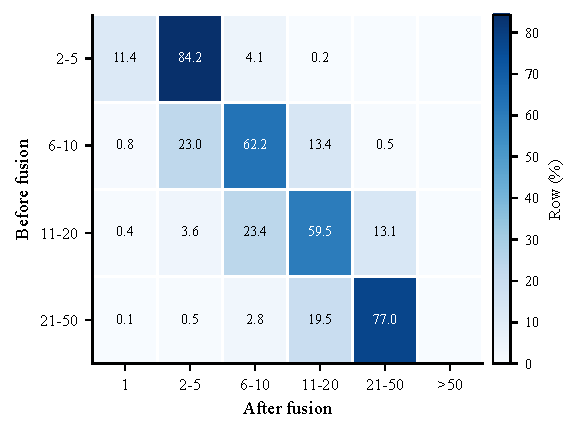
\includegraphics[draft=false,width=0.90\columnwidth]{fig3_rank_transition_heatmap_only.pdf}
% \caption{Rank transition on the high-ranked failure subset. Rows and columns denote the ground-truth rank buckets before and after global-local fusion, respectively; each row is normalized to 100\%.}
% \label{fig:rank_movement}
% \end{figure}

\subsection{Parameter Sensitivity Analysis (RQ4)}
\label{sec:rq4_params}

We analyze the sensitivity of \method{} to two refinement-stage hyperparameters on JavaScript: the failure-calibrated supervision weight \(\lambda_f\) and the retained candidate size \(m\). Starting from the default configuration in Section~\ref{sec:impl}, we vary one hyperparameter at a time while keeping the others unchanged. Fig.~\ref{fig:param_sensitivity} reports the corresponding MRR, R@1, R@5, and R@10 results under each tested configuration.

As shown in Fig.~\ref{fig:param_sensitivity}, \method{} remains stable across different values of \(\lambda_f\). When \(\lambda_f\) varies from 0.25 to 0.65, Fusion MRR stays within a narrow range from 79.00\% to 79.20\%, while R@1, R@5, and R@10 also exhibit only minor fluctuations. The best Fusion MRR is achieved at \(\lambda_f=0.45\), tied with \(\lambda_f=0.65\), while the default setting keeps the supervision strength moderate without sacrificing stability.

For the retained candidate size \(m\), the overall trend is similarly stable, but the figure also reveals a clearer performance pattern. When only two candidates are retained, the model achieves relatively lower performance. Increasing \(m\) from 2 to 8 improves Fusion MRR from 78.92\% to 79.20\%, while R@1 also increases from 69.37\% to 69.80\%. When \(m\) is too small, the retained candidates may not sufficiently cover diverse high-ranked errors; when \(m\) becomes too large, additional candidates may introduce weaker refinement signals. Further increasing \(m\) to 16 or 32 brings only marginal changes. Although larger \(m\) values slightly improve R@5 and R@10, they do not yield further gains in Fusion MRR within the explored range.

\begin{figure}[!t]
\centering
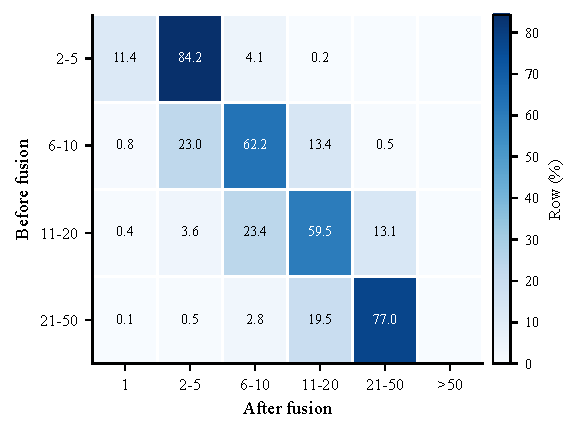
\includegraphics[draft=false,width=\columnwidth]{fig3_rank_transition_heatmap_only.pdf}
\caption{Rank transition on the high-ranked failure subset. Rows and columns denote the ground-truth rank buckets before and after global-local fusion, respectively; each row is normalized to 100\%.}
\label{fig:rank_movement}
\end{figure}


\begin{figure}[!t]
\centering
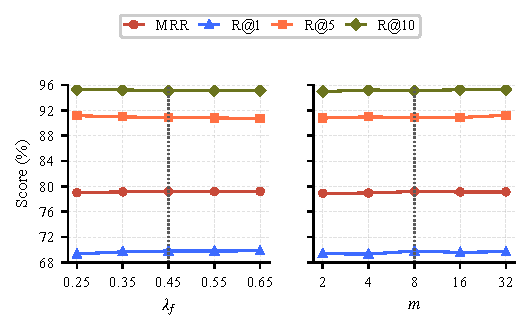
\includegraphics[draft=false,width=\columnwidth]{param_analysis_2panel_revised.pdf}
\caption{Parameter sensitivity on JavaScript. The left panel varies the failure-calibrated supervision weight \(\lambda_f\), and the right panel varies the retained candidate size \(m\).}
\label{fig:param_sensitivity}
\end{figure}

% \noindent\textbf{Answer to RQ4.}
% \method{} remains stable across the tested values of \(\lambda_f\) and \(m\), suggesting that its performance is not tied to a fragile hyperparameter choice.
% \answerbox{RQ4}{\method{} remains stable across the tested values of \(\lambda_f\) and \(m\), suggesting that its performance is not tied to a fragile hyperparameter choice.}
\answerbox{RQ4}{\method{} remains stable across the tested values of \(\lambda_f\) and \(m\). The small performance variations indicate that the refinement stage is not overly sensitive to either hyperparameter.}

\section{Related Work}

\subsection{Neural Code Search}

Code search aims to retrieve code snippets that match the intent of a natural language query. 
Early information-retrieval-based methods rely on lexical matching, structural information, or API-aware query expansion to estimate query-code relevance~\cite{Sourcerer,Portfolio,CodeHow}. 
Neural methods further learn distributed representations of code and natural language, such as DeepCS and UNIF~\cite{DeepCS,UNIF}. 
Later studies incorporate overlap signals, structural features, intermediate representations, and meta-learning strategies to improve semantic matching~\cite{OCoR,TabCS,CSRS,TranCS,CDCS}. 
With the development of pre-trained code models, CodeBERT, GraphCodeBERT, UniXcoder, SynCoBERT, CodeT5, and PLBART have become widely used backbones for code understanding and code search tasks~\cite{CodeBERT,GraphCodeBERT,UniXcoder,SynCoBERT,CodeT5,PLBART}.
Recent work also studies hybrid and cross-language code retrieval, where different modalities and programming languages introduce additional representation challenges~\cite{UniCoR}. 
These studies mainly improve model architectures, pre-training objectives, or representation spaces. 
In contrast, \method{} is complementary to backbone-oriented methods: it starts from an already trained retriever and refines the ranking behavior exposed by its own high-ranked candidates.

\subsection{Contrastive Learning for Code Search}

Contrastive learning has been widely adopted for code search because it aligns semantically related query-code pairs and separates irrelevant ones in the representation space. 
CodeRetriever introduces unimodal and bimodal contrastive learning for code-text representation learning~\cite{CodeRetriever}. 
CoCoSoDa improves contrastive code search through soft data augmentation, a momentum encoder, and multimodal contrastive learning~\cite{CoCoSoDa}. 
Corder constructs semantically equivalent code snippets through program transformations and learns code representations with contrastive objectives~\cite{Corder}. 
ContraCode and ContraBERT also show that contrastive learning can provide useful self-supervision for robust code representation learning~\cite{ContraCode,ContraBERT}. 
% MCodeSearcher further explores multi-view contrastive learning for code search~\cite{MCodeSearcher}.
These studies demonstrate the effectiveness of contrastive supervision for learning discriminative query-code representations. 
However, their objectives mainly optimize general representation separation, while the high-ranked candidates produced by the trained retriever are not explicitly used as refinement signals. 
\method{} follows the contrastive learning paradigm, but its refinement signal is constructed from model-induced high-ranked candidates, making the training objective more closely related to the final ranking behavior.

\subsection{Hard Negative Mining and Retrieval Refinement}

Hard negative mining improves contrastive supervision by constructing challenging mismatched query-code pairs. In code search, existing methods often select hard or informative samples using lexical overlap, representation similarity, uncertainty estimation, ranking signals, relevance objectives, or predefined mining rules~\cite{AAAIUA,CoCoHaNeRe,HedgeCode,R2PS}. Similar issues have also been studied in dense retrieval, where hard negatives and denoised negative sampling are used to reduce the mismatch between training samples and test-time ranking behavior~\cite{DPR,ANCE,HardNegDR,RocketQA}. For example, dense retrieval studies show that negatives retrieved from an index can better approximate the candidates encountered during search than uniformly sampled negatives. These findings are consistent with our empirical observation that random negatives and static hard negatives do not fully characterize inference-time high-ranked candidates. Nevertheless, many hard-negative strategies still operate as training-time proxies: a candidate can be difficult under a mining rule but may not be the candidate that suppresses the ground-truth code in the final ranked list. ReFCode differs by constructing refinement candidates from the retriever's own ranked results, linking the training signal to inference-time ranking behavior rather than only to predefined training-time mining heuristics. This distinction is important for high-ranked candidate spaces in practical retrieval settings, where the ground-truth code and misleading candidates are often already close in the retriever's global representation space at inference.

\subsection{Fine-Grained Query-Code Matching}

Fine-grained query-code matching is important for distinguishing snippets that are globally similar but functionally different. 
FcarCS introduces fine-grained co-attentive representation learning to capture interdependent relationships between code and natural language queries~\cite{FcarCS}. 
Other methods use cross-modal encoding and co-attention mechanisms to model detailed query-code interactions~\cite{FineGrainedCS}. 
HedgeCode defines a code-text relevance detection task and uses hedging contrastive learning to capture fine-grained differences~\cite{HedgeCode}. 
In broader information retrieval, ColBERT introduces late interaction to preserve token-level representations and perform MaxSim-based matching~\cite{ColBERT}. 
These interaction-based methods are effective for close candidates because they preserve more local evidence than a single pooled representation. 
However, applying full token-level interaction to the entire codebase is expensive and can weaken the practical advantage of dual-encoder retrieval. 
\method{} follows the same intuition that local evidence is useful for disambiguating semantically close candidates, but applies local interaction only over compact top-\(K\) candidates after global retrieval. 
This design keeps large-scale retrieval in the dual-encoder form while using local matching evidence to refine the final ordering of difficult high-ranked candidates returned by the global retriever.

\section{Threats to Validity}

\subsection{Dataset and Ground-Truth Validity}

Our experiments are conducted on the six-language CodeSearchNet benchmark, which enables systematic comparison across programming languages and retrieval methods. 
However, real-world software development environments may differ from CodeSearchNet in repository scale, project structure, query formulation, and language distribution. 
In addition, CodeSearchNet treats the paired code snippet as the ground-truth result for a query, while real queries may correspond to multiple semantically correct implementations. 
Thus, a high-ranked unpaired candidate may still be semantically relevant in some cases. 
This annotation ambiguity may affect the interpretation of model-induced high-ranked candidates and ranking errors. 
Therefore, the failures studied in this paper should be understood as failures with respect to benchmark annotations rather than absolute semantic errors in all real-world contexts. 
To reduce over-interpretation, our analysis focuses on retrieved-but-mis-ranked cases and aggregate ranking behavior rather than making fine-grained relevance claims for every unpaired candidate in the benchmark.

\subsection{Baseline and Implementation Validity}

We compare \method{} with representative methods, including CodeBERT, GraphCodeBERT, UniXcoder, SynCoBERT, CodeRetriever, CoCoSoDa, HedgeCode, and UA-HN. 
Although these methods are evaluated on CodeSearchNet with the same evaluation metric, differences in preprocessing, implementation details, hyperparameter settings, and candidate pool construction may affect absolute performance values. 
This threat is particularly relevant when comparing against published results reported by prior work. 
To reduce this threat, we include widely used and recent strong baselines, and conduct internal ablation studies and ranking behavior analysis under a unified experimental setting. 
Therefore, the main evidence for the effectiveness of \method{} comes not only from comparisons with published baselines, but also from controlled comparisons with the initial retriever and ablation variants under the same experimental setting and evaluation protocol.

\subsection{Initial Retriever and Hyperparameter Sensitivity}

\method{} relies on an initial retriever to produce model-induced high-ranked candidates, and different initial retrievers may produce different candidate distributions. 
The framework also involves several implementation choices, including the size of the harvested candidate pool, the number of retained failure candidates, the weight of the local interaction objective, and the global-local fusion coefficient. 
These choices may affect the magnitude of the observed improvements. 
To reduce this threat, we select checkpoints on the validation set and use the same fusion coefficient \(\alpha=0.5\) across all languages for test evaluation. 
We further conduct parameter sensitivity analysis on JavaScript for two refinement-stage hyperparameters, namely the failure-calibrated supervision weight \(\lambda_f\) and the retained candidate size \(m\). 
However, this analysis covers only one representative language and two key hyperparameters, and does not exhaustively search all candidate-pool sizes, loss weights, or fusion coefficients across all languages.

\section{Conclusion and Future Work}

In this paper, we study high-ranked ranking errors in neural code search. 
We first conduct an empirical study and find that strong retrievers still produce retrieved-but-mis-ranked cases, and that model-induced high-ranked candidates are not sufficiently captured by conventional static hard negatives. 
Based on this finding, we propose \method{}, a failure-calibrated dual-granularity refinement framework for code search. 
Experiments on the six-language CodeSearchNet benchmark show that \method{} achieves the best average MRR among all compared methods, while ablation studies and ranking behavior analysis further validate the effectiveness of failure-calibrated supervision, local interaction, and global-local fusion.

In future work, we plan to evaluate ReFCode under more realistic code search scenarios, larger repositories, and more retrieval backbones. 
We will also explore more efficient local interaction mechanisms and candidate-quality estimation strategies for more robust ranking refinement in complex and large-scale code search settings.

\section{Data Availability}

The dataset used in this paper is based on the publicly available CodeSearchNet benchmark. 
The source code, configuration files, and processed intermediate candidate files of ReFCode are available in our anonymized repository: \url{https://anonymous.4open.science/r/ReFCode-4955}. 
The repository also includes scripts for candidate harvesting, refinement training, reranking, and evaluation to facilitate reproduction of the main experiments reported in this paper.

\clearpage

\bibliographystyle{IEEEtran}
\bibliography{references}

\end{document}
